Có 3 loại mối quan hệ giữa các bối cảnh bị giới hạn là:

\begin{itemize}

\item Mối quan hệ đối xứng (Symmetric Relationship)

\textbf{Mô tả:} Thể hiện sự tương tác 2 chiều giữa 2 bối cảnh bị giới hạn .

\item Mối quan hệ bất đối xứng (Asymmetric Relationship)

\textbf{Mô tả:} Thể hiện sự tương tác 1 chiều giữa 2 các bối cảnh bị giới hạn .

\item Mối quan hệ 1 - nhiều (One to Many Relationship)

\textbf{Mô tả:} Thể hiện sự tương tác 1 chiều giữa 1 bối cảnh bị giới hạn với nhiều bối cảnh bị giới hạn khác.

\end{itemize}

\begin{figure}[H]

\centering

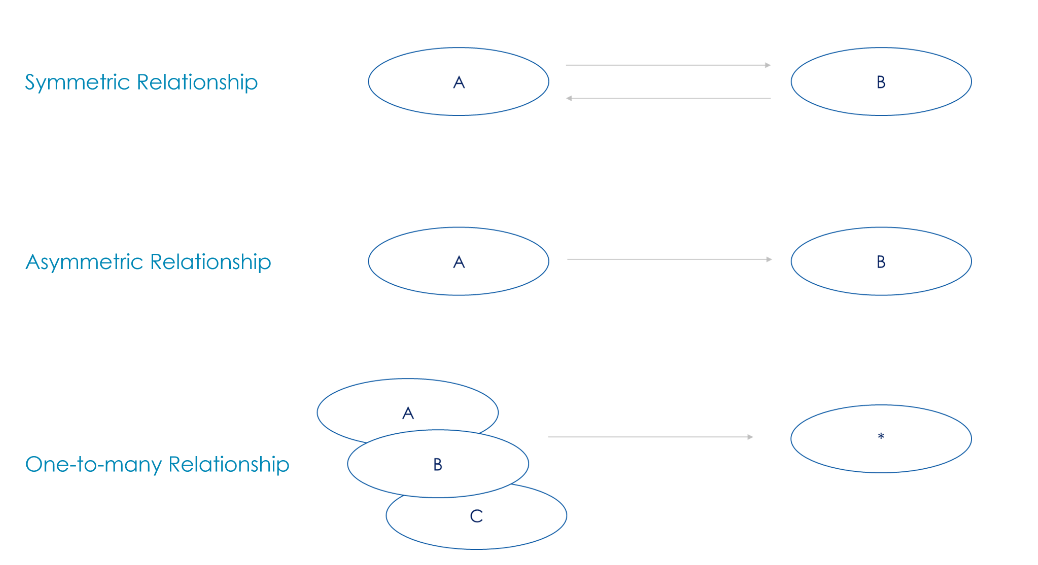
\includegraphics[scale = 0.5]{pictures/cac_moi_quan_he_boi_canh_gioi_han/main.png}

\caption{Các mối quan hệ bối cảnh bị giới hạn}

\end{figure}

